\chapter{Introduction}
\label{chap1}

Embedded computer vision methods are increasingly used to gather and interpret information from outdoor environments. The data derived from this analysis are used for a plethora of applications, including autonomous navigation, vision based-localization, precision agriculture, obstacle detection and more. However, the reliability of these applications depends heavily on data clarity. In particular, illumination variability and dynamic viewing conditions significantly impact the the quality of the captured data and, consequently, the resulting algorithm performance. 

Among these challenges, variations in viewing conditions are particularly prominent in exterior environments, where solar zenith angle, associated shadows and weather phenomena are not controllable parameters \cite{edges_under_illumvar, dl_low_light, impact_of_sunlight_conditions, fruit_detection_illvar, effect-time-day}. These natural obstacles, along with current technological limitations, such as  geometry dependent sensors unable to be efficiently calibrated for different illumination scenarios \cite{color_consistency}, do hinder proper functionality even further. As a result, frames depicting the same object under varying viewing conditions can lead to inconsistent algorithmic decision-making, as the object's appearance and fundamental properties - such as its detected boundaries, visibility and estimated reflectance of its surface -  appear altered \cite{edges_under_illumvar, dl_low_light, impact_of_sunlight_conditions}.

For these systems to fulfill their purpose successfully, they must be robust and somewhat agnostic to unavoidable environmental changes. A common practice in previous outdoor computer vision surveys was to mitigate the effects of directional light, which causes shadows and illumination imbalances, by relying on diffuse lighting \cite{impact_of_sunlight_conditions, ps_cloudy, autonomous_agriculture}. Despite the demonstrably improved performance of algorithms under diffuse lighting, most of modern embedded computer vision systems cannot be designed to operate exclusively under such conditions, as non-robust systems' susceptibility to dynamic weather phenomena and illumination conditions can lead to immediate safety hazards due to unstable segmentation \cite{safetyhaz-cv}, failure of reliable monitoring of civil infrastructure's structural integrity \cite{bridges, construction-site} and inconsistent measurements in radiometric applications \cite{impact_of_sunlight_conditions, effect-time-day, variable-illum-vi}. This superior performance under diffuse lighting, though, directly inspires a way of mitigating the effects of illumination variability.

Another approach commonly encountered in the literature is the use of machine learning methods, either for restoring images affected by the previously mentioned challenges \cite{dl_low_light, dl-img-rest, macgan}, or for recovering radiometric quantities, distorted by environmental conditions \cite{illum-correction, rfg-change-detect}. Such approaches can provide a reliable solution, provided there are sufficient representative training data. However, the hardships of acquiring suitable data were expressed in multiple works \cite{dl-img-rest, rfg-change-detect}. As a result, several studies have relied, at least partly, on synthetic data \cite{dl-img-rest, macgan}.

\section{Scope of the Thesis}

This study focuses on addressing one of the aforementioned side-effects of illumination variability: its impact on the perceived reflectance of an examined surface. Reflectance is typically measured directly using a spectrophotometer or estimated, with some degree of error, using a digital camera, properly calibrated for capturing scene luminance \cite{luminance-cal-camera, rp-luminance-cmaera} alongside an irradiance spectrometer \cite{drones-reflectance}. Predictably, this error could grow even larger under unideal lighting conditions.

I examined this phenomenon through its appearance in a specific precision agriculture application: the calculation of the Green Red Vegetation Index (GRVI) on parts of a studied wheat field.  Specifically, the measured GRVI values frequently appear inconsistent, depending on dynamic weather phenomena, the solar zenith angle and the observer's position. This is mostly attributed to the anisotropic BRDF of the crop canopy, making parts of the field appear less illuminated than the rest, even if the incident radiant flux remains uniform across the field \cite{impact_of_sunlight_conditions, brdf}. Furthermore, even when the sun is at solar zenith, minimizing the uneven distribution of reflected radiation, cast shadows persist and continue to affect the estimated reflectance. 

A method that was proven effective was the collection of incident radiation flux and luminance data under overcast lighting conditions, as this naturally mitigates the influence of the sun position, viewing angle  and cast shadows. Two representative examples of this effect are provided by Ishihara et al. (2015) and Rasmussen et al. (2016). In the study of Ishihara et al. (2015) \cite{impact_of_sunlight_conditions}, NDVI and GRVI exhibited regression slopes of up to 0.005 and 0.0054 per solar zenith angle (SZA) degree, respectively, under clear-sky conditions, whereas under cloudy conditions almost all slopes remained bellow 0.001 per degree, indicating greater measurement stability. Similarly, in the work of Rasmussen et al. (2016) \cite{cons-grade-cams}, it was observed that changes in brightness caused by viewing angle did not affect perceived vegetation indices' values under cloudy weather conditions, contrary to clear-sky conditions. Directional reflectance effects caused by light's directionality and unisotropic BRDF of crops' canopy were also mitigated under cloudy weather conditions, while the lack of shadows eliminates significant illumination variations.

Since, though, plant monitoring cannot be restricted only to periods when the weather conditions are ideal, the information gathered during these periods can serve as a reference baseline. By using this baseline to train a machine learning regression model, the system learns to map measurements acquired under non-ideal outdoor conditions to their corresponding reference values. Once trained, the model can estimate what the perceived reflectance would have been under diffuse lighting conditions, allowing consistent monitoring of the plants under a wider range of observation conditions. This pipeline is depicted in Figure ~\ref{ml-pipeline-1}.

\begin{figure}[htb]
    \centering

    \begin{subfigure}{1\textwidth}
        \centering
        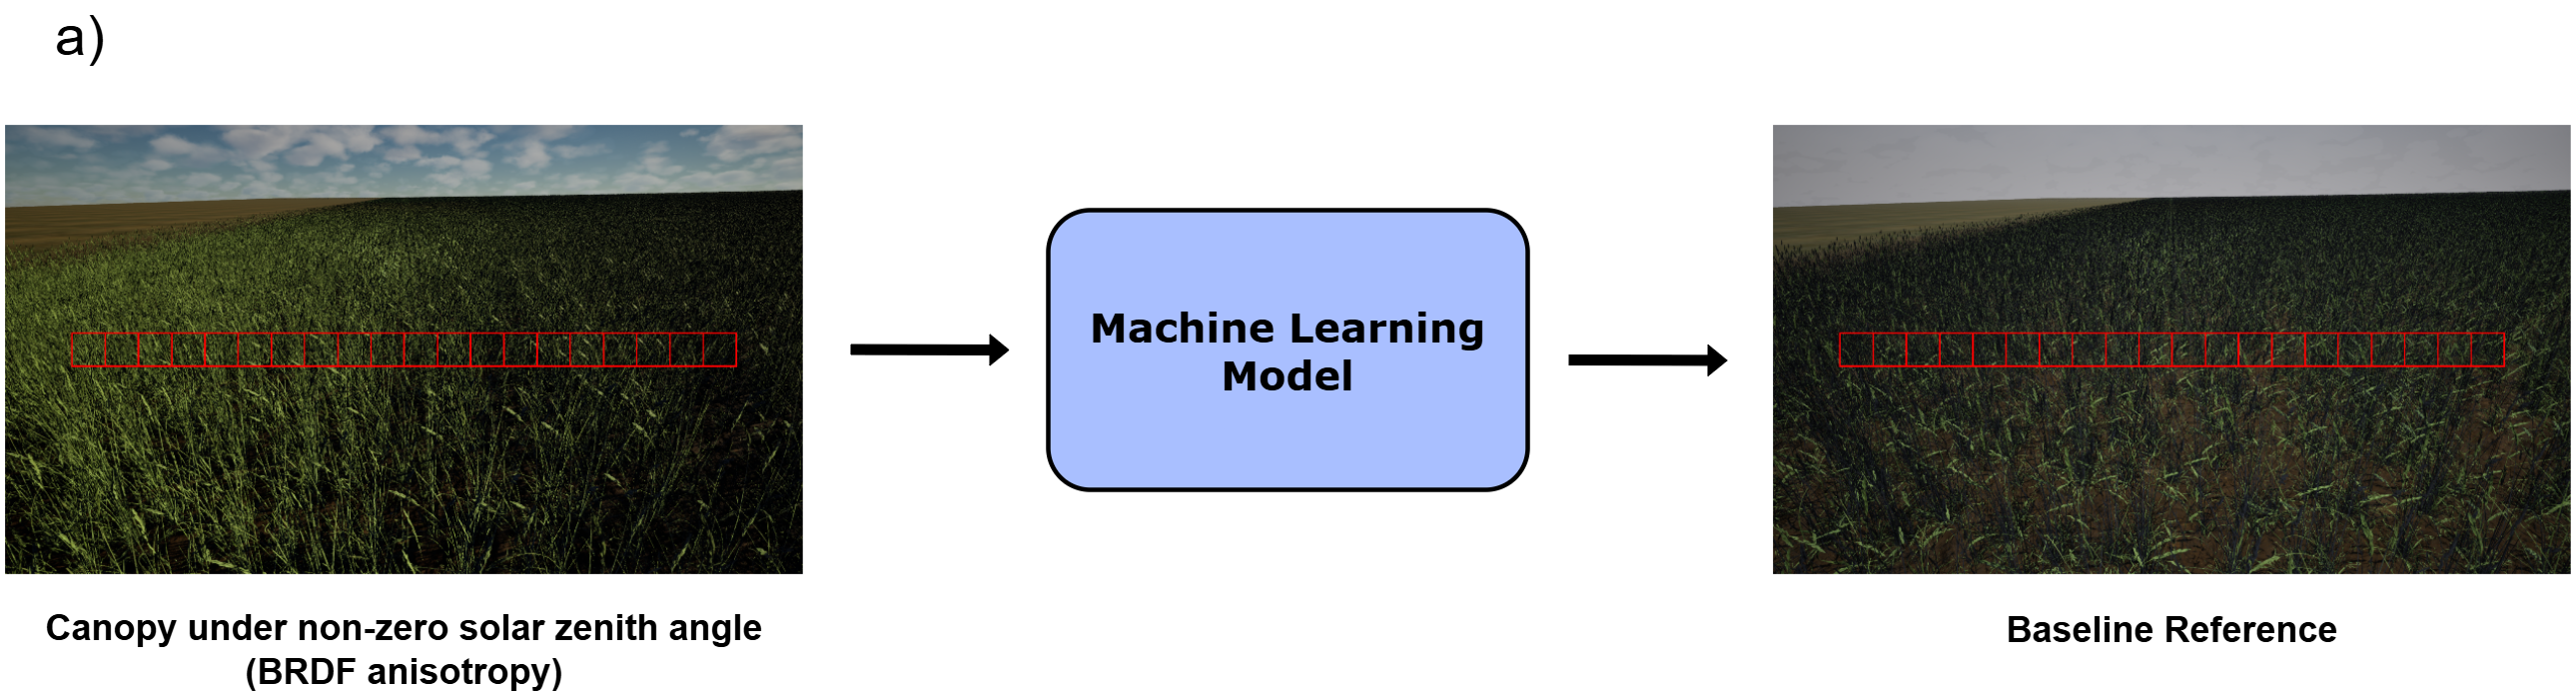
\includegraphics[width=\textwidth]{images/brdf-to-gt.png}
        \caption{First image caption}
        \label{fig1}
    \end{subfigure}

    \vspace{0.5cm}

    \begin{subfigure}{1\textwidth}
        \centering
        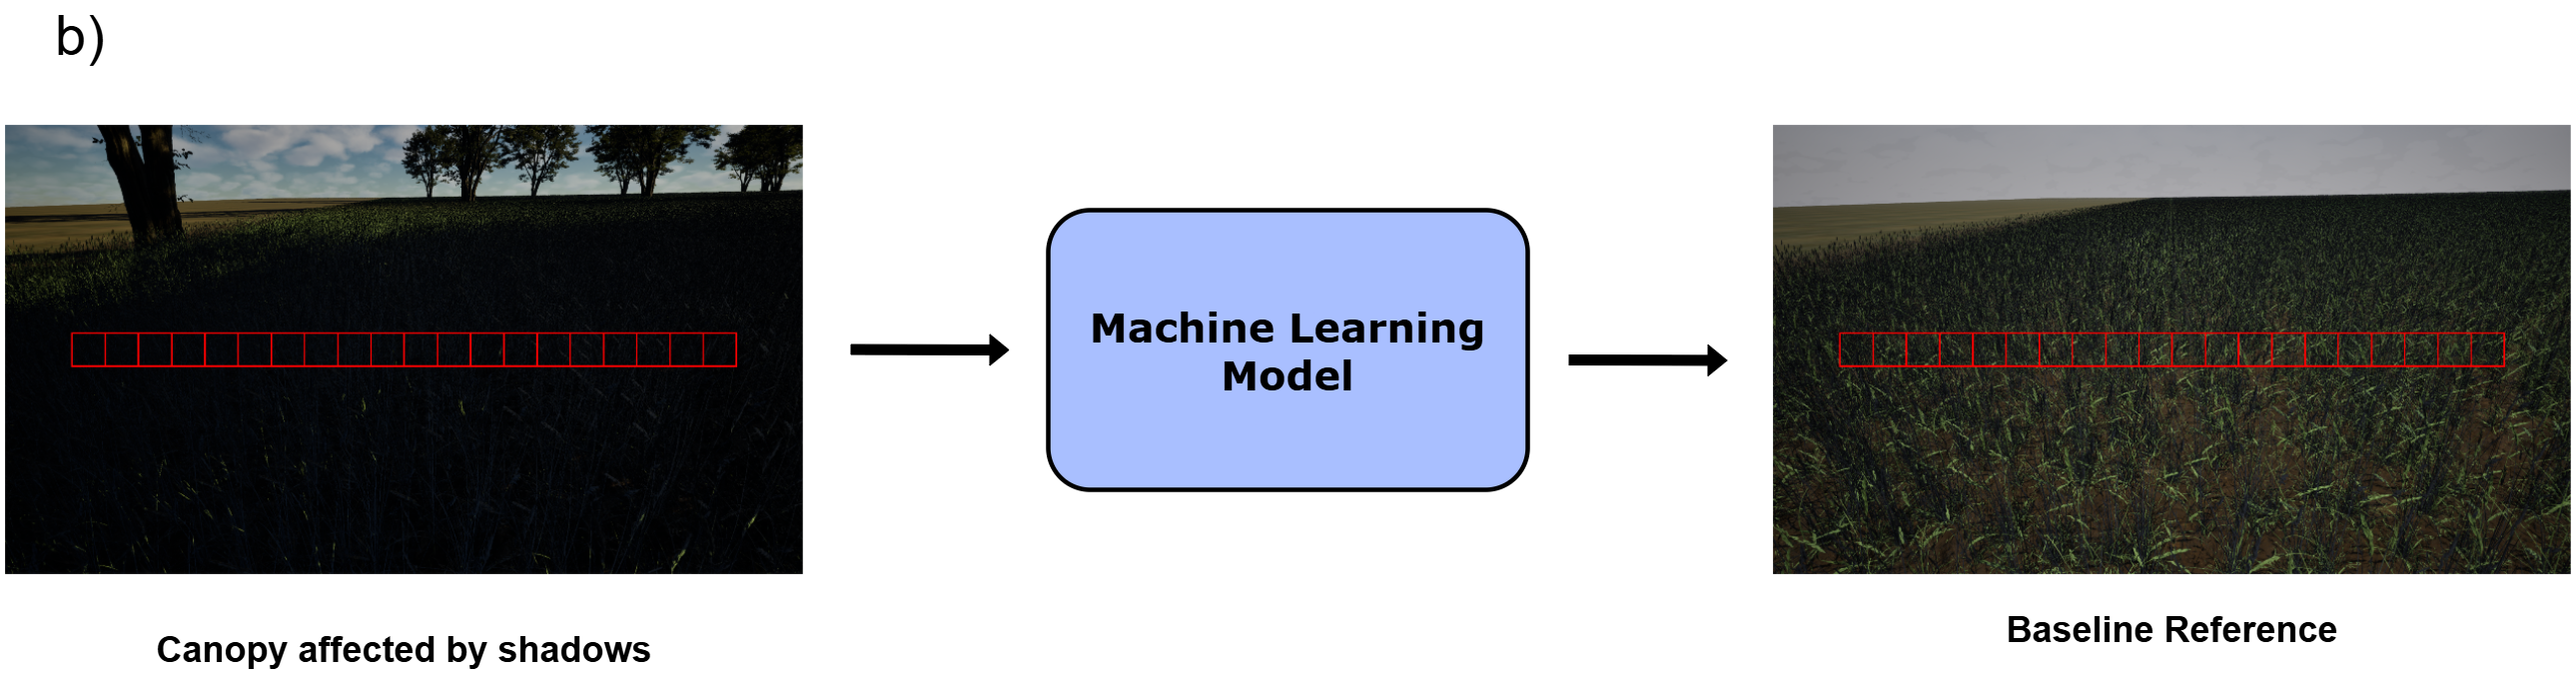
\includegraphics[width=\textwidth]{images/trees-to-gt.png}
        \caption{Second image caption}
        \label{fig2}
    \end{subfigure}

    \caption{The two primary sources of error in this study, excluding errors originating from the sensors used: a) Wheat canopy's anisotropic BRDF, making the sun-sensor-field geometry relevant to the calculated GRVI value and b) The effect of shadows. These factors introduce noise to the perceived material reflectances, and therefore GRVI. Machine learning will be used for approximating the GRVI value under ideal illumination conditions, given the values measured under non-ideal conditions.}
    \label{ml-pipeline-1}
\end{figure} 

The inclusion of machine learning and need for training data introduce an additional challenge to the implementation of the proposed system. Constructing a training dataset would require images captured under ideal weather conditions at different stages of the crops’ growth, serving as the ground truth data which the model will attempt to approach as an output, along with images of the same scenes under non-ideal weather conditions. Collecting such data could be both time- and cost-inefficient, considering the stochastic nature of the weather phenomena.

To overcome this data acquisition barrier, a digital twin of a crop field was developed, becoming the primary data source. By offering control over lighting and atmospheric conditions, material properties and crops growth, digital twins provide a highly robust alternative to physical data collection. Furthermore, advancements in modern graphics, specifically regarding the capacity to render photorealistic digital environments, ensure the viability of synthetic scenes as accurate replications of their real-world counterparts. 


By modeling the studied sources of error influencing GRVI measurements within the digital twin, their individual and combined effects can be characterized and learned by ML models, enabling substantial reduction in measurement variability caused by external conditions. While regressing to values captured under ideal weather conditions removes noise attributed to factors originating from the weather, several other environmental and technological factors persist, including improperly calibrated sensors, the existence of soil in the background and outliers captured during the data collection of the reference baseline. To address these remaining challenges, a second training pipeline is proposed, aiming to approximate directly the GRVI that was assigned to the materials of the virtual meshes before their deployment (Figure ~\ref{ml-pipeline-2}).

\begin{figure} [htb]
    \centering
    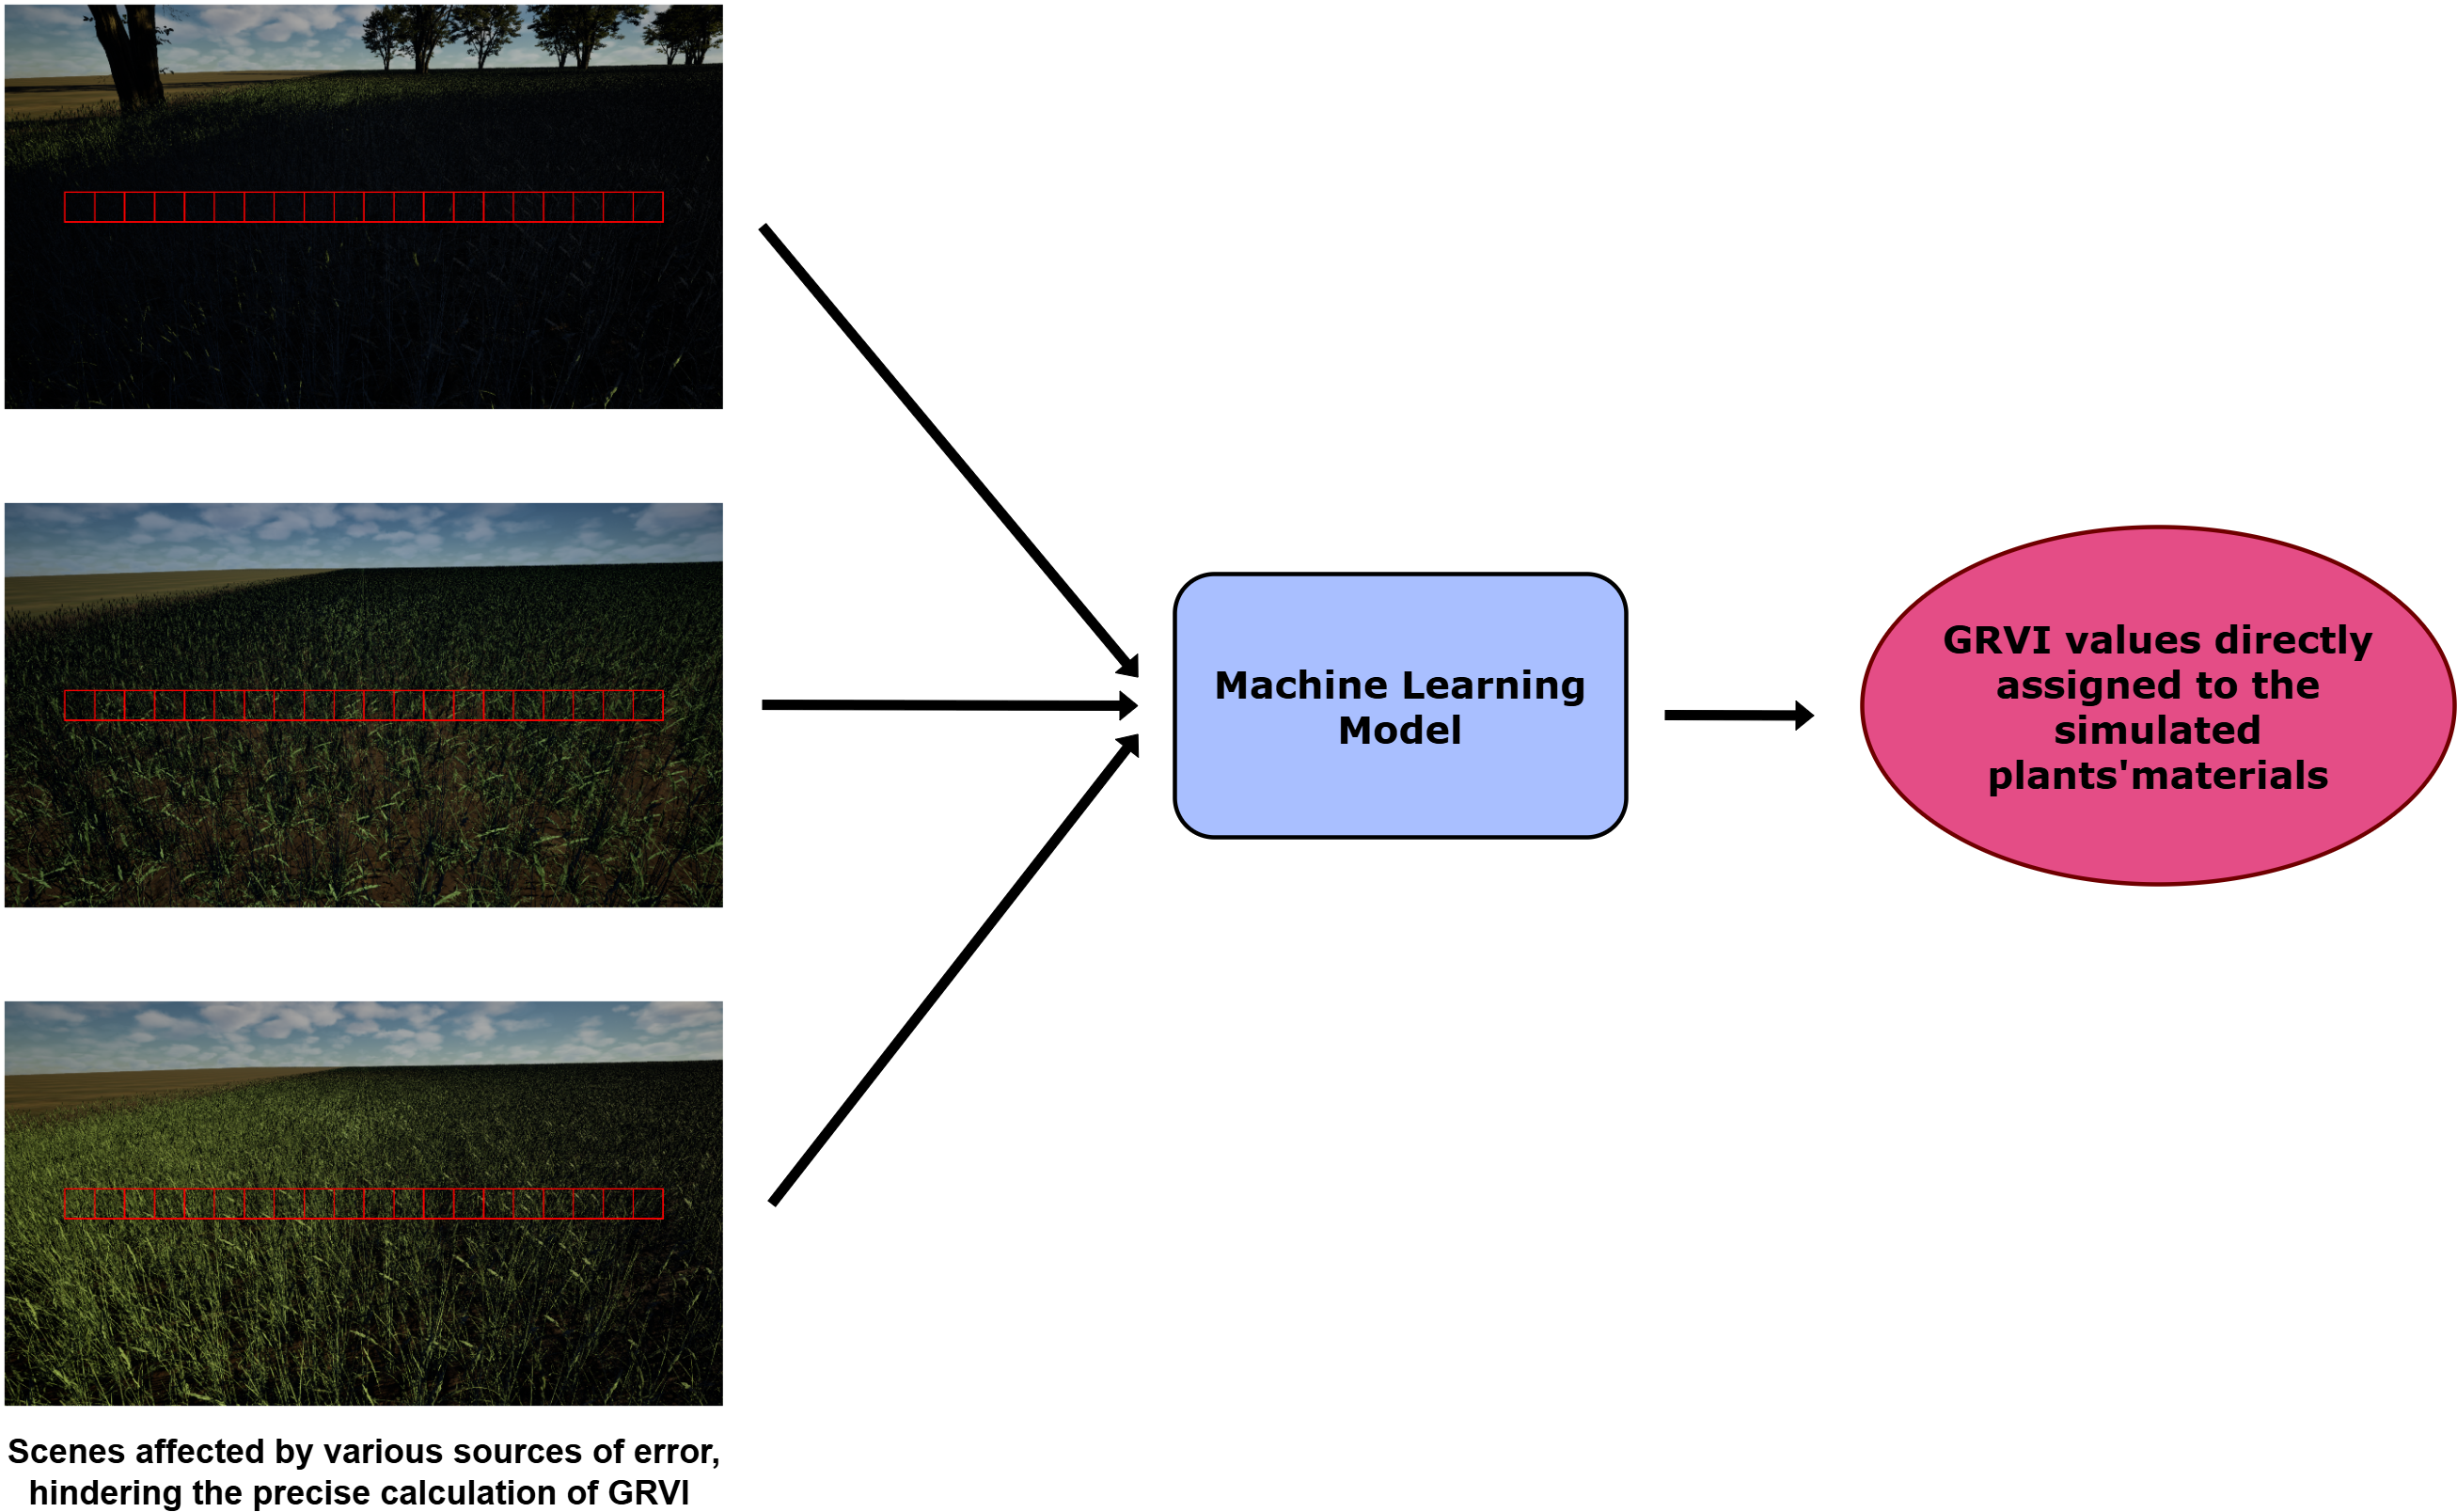
\includegraphics[width=1\linewidth]{images/truegt-pipeline.png}
    \caption{The proposed pipeline for mitigating related to both atmospheric noise and overall environmental and technological factors.}
    \label{ml-pipeline-2}
\end{figure}

\subsection{Contribution}
The main contributions of this work are listed below:

\begin{enumerate}
\item An analytical study identifying the primary factors that cause the perceived reflectance of surfaces to deviate from their actual values.  
\item The development of a photorealistic digital twin of a wheat field in Unreal Engine, specifically engineered to accurately replicate these factors.
\item The creation of tools for automated data collection, ensuring that indexed data (linear images of the scene, the associated illuminance meter readings and camera information etc.) are all both spatially and numerically  aligned.
\item The preprocessing and structuring of the synthetic data into a comprehensive dataset for machine learning applications. 
\item The training and evaluation of various machine learning models on the dataset, designed to regress to GRVI values not affected by weather phenomena, light directionality and viewing geometry. 
\item The identification of an optimal model that successfully balances high predictive performance with low computational overhead, ensuring its viability for edge device deployment.
\item The implementation of a secondary set of machine learning models, designed to approximate GRVI values completely isolated from any source of noise, again, with hardware efficiency in mind. 
\end{enumerate}


\section{Thesis Structure}

This thesis is organized into eight main chapters. In Chapter~\ref{chap1} I define the core challenges this study addresses, introduce the proposed methodological solutions and outline the primary contributions. In Chapter~\ref{chap2} I establish the theoretical foundation by introducing the reader to several key concepts that recur throughout this work. Such concepts include the definition of the spectrometry mechanisms explored, the introduction to Unreal Engine and its involvement in creating synthetic data, and the fundamental machine learning principles used to train the predictive models. Chapter~\ref{chap3} ...

Chapters 4, 5 and 6 are dedicated to presenting the methodology I followed for addressing the identified challenges. In Chapter~\ref{chap4} I detail the implementation of the digital twin in Unreal Engine and introduce the methods used within the digital environment for acquiring information regarding the calculation of a surface's reflectance. In Chapter~\ref{chap5} I describe the stages of the data collection pipeline and the preprocessing of the accumulated data for machine learning applications.